\documentclass[conference]{IEEEtran}
\IEEEoverridecommandlockouts
\usepackage{cite}
\usepackage{amsmath,amssymb,amsfonts}
\usepackage{algorithmic}
\usepackage{graphicx}
\usepackage{textcomp}
\usepackage{xcolor}
\usepackage{booktabs}
\def\BibTeX{{\rm B\kern-.05em{\sc i\kern-.025em b}\kern-.08em
    T\kern-.1667em\lower.7ex\hbox{E}\kern-.125emX}}

\begin{document}

\title{Vision-Based Connect-4 Robot: Image Processing Pipeline\\
for Autonomous Game-State Extraction and Motor Control}

\author{%
\IEEEauthorblockN{Andrew Abdelmalak}
\IEEEauthorblockA{\textit{Dept.\ of Mechatronics Engineering}\\
\textit{German University in Cairo}\\
Cairo, Egypt\\
andrew.abdelmalak@student.guc.edu.eg}
\and
\IEEEauthorblockN{Daniel Boules}
\IEEEauthorblockA{\textit{Dept.\ of Mechatronics Engineering}\\
\textit{German University in Cairo}\\
Cairo, Egypt\\
daniel.boules@student.guc.edu.eg}
\and
\IEEEauthorblockN{David Girgis}
\IEEEauthorblockA{\textit{Dept.\ of Mechatronics Engineering}\\
\textit{German University in Cairo}\\
Cairo, Egypt\\
david.girgis@student.guc.edu.eg}
\and
\IEEEauthorblockN{Kirolous Kirolous}
\IEEEauthorblockA{\textit{Dept.\ of Mechatronics Engineering}\\
\textit{German University in Cairo}\\
Cairo, Egypt\\
kirolous.kirolous@student.guc.edu.eg}
\and
\IEEEauthorblockN{Samir Yacoub}
\IEEEauthorblockA{\textit{Dept.\ of Mechatronics Engineering}\\
\textit{German University in Cairo}\\
Cairo, Egypt\\
samir.yacoub@student.guc.edu.eg}
\and
\IEEEauthorblockN{Youssef Salama}
\IEEEauthorblockA{\textit{Dept.\ of Mechatronics Engineering}\\
\textit{German University in Cairo}\\
Cairo, Egypt\\
youssef.salama@student.guc.edu.eg}
}

\maketitle

\begin{abstract}
This paper presents the design and implementation of an autonomous Vision-Based
Connect-4 Robot, a mechatronic system that integrates computer vision,
embedded computing, and robotic actuation. An RGB camera acquires frames of
a standard 7\(\times\)6 Connect-4 grid; a Python/OpenCV processing
pipeline performs geometric normalization, intensity conditioning, and noise
suppression; and two scalar image features drive closed-loop motor commands
transmitted over a serial link to an Arduino-controlled actuation stage.
The full pipeline has been validated on a Raspberry~Pi~4 (4~GB) and benchmarked
against a laptop platform. Execution times per operation range from
0.73~ms to 8.47~ms on the Raspberry~Pi. Output image quality is
bit-for-bit identical on both platforms. The mechanical assembly,
modeled in SolidWorks, uses a magazine-and-slide dispensing mechanism
with a servo-controlled gate for column selection.
\end{abstract}

\begin{IEEEkeywords}
Connect-4, computer vision, image processing, Raspberry Pi,
closed-loop motor control, OpenCV, SolidWorks, Arduino
\end{IEEEkeywords}

% ─────────────────────────────────────────────────────────────────────────────
\section{Introduction}
% ─────────────────────────────────────────────────────────────────────────────

Autonomous game-playing robots are compelling mechatronic testbeds because they
demand tightly integrated perception, cognition, and actuation operating in a
real-time loop~\cite{Zubek2021}. The robot described here targets Connect-4, a
two-player, zero-sum game in which the first player to align four same-colored
discs—horizontally, vertically, or diagonally—wins. Tokens fall under gravity
once released above the correct column, which simplifies the end-effector
requirement: the arm must achieve repeatable lateral positioning over each
column entry with an error smaller than half the column pitch
(\(\approx 20\)~mm for a standard board), but need not execute a
grasp-and-insert motion.

The system comprises three integrated subsystems:
\begin{enumerate}
\item \emph{Perception}: a Pi Camera~V2 capturing overhead RGB frames,
  followed by an OpenCV-based preprocessing pipeline;
\item \emph{Computation}: a Raspberry~Pi~4 (4~GB) running Python, extracting
  image features and transmitting serial commands;
\item \emph{Actuation}: an Arduino~Uno receiving scalar commands and driving
  NEMA~17 stepper motors via L298N H-bridge drivers, with a servo-controlled
  gate for column selection.
\end{enumerate}

This paper reports the system through Milestone~2: the image processing
pipeline has been implemented and benchmarked, the mechanical assembly has been
designed in SolidWorks, and the electrical architecture has been validated in
Proteus simulation. The game-solving AI (minimax with alpha-beta pruning) and
real-time closed-loop integration represent the next development phase and are
not yet implemented.

% ─────────────────────────────────────────────────────────────────────────────
\section{Related Work}
\label{sec:related}
% ─────────────────────────────────────────────────────────────────────────────

\subsection{Board Detection and Game-State Extraction}

Extracting a complete game state from a camera image is the foundational
perceptual task. W\"{o}lflein and Arandjelovi\'{c}~\cite{Wolflein2021} proposed
a modular CNN pipeline for chess recognition—automated corner localization,
homographic perspective rectification, and per-cell CNN inference—achieving
greater than 98\% per-square occupancy accuracy. This modular structure
transfers directly to a 7\(\times\)6 Connect-4 grid by replacing the
six-class piece classifier with a three-class one (red token, yellow token,
empty cell). Rezaei and Raihan~\cite{Rezaei2023} extended this line with a
fully end-to-end model that eliminates the explicit rectification stage,
reducing processing latency by removing the critical failure mode of missed
corner detections.

\subsection{Token Detection and Color Segmentation}

Reliable token-color identification distinguishes Connect-4 perception from
monochromatic chess recognition. Ambient illumination in a laboratory
environment can shift the apparent token hue by 20--40 degrees in RGB space,
making the Hue--Saturation--Value (HSV) color space the de-facto standard for
illumination-tolerant segmentation~\cite{Park2024}. An adaptive HSV pipeline
evaluated on pick-and-place tasks with objects matching the Connect-4 color
palette (red, yellow, green, blue) maintained detection accuracy above 97\%
under illuminance levels from 200 to 1200~lux~\cite{Park2024}. The
Connect-4-specific study in~\cite{Zubek2021} used HSV thresholding on a
per-cell region of interest at 10~Hz on embedded hardware, providing a
validated baseline for game-state updates.

\subsection{Manipulator Hardware Design}

The open-source chess robot in~\cite{Abarkan2024} demonstrated a three-axis
Cartesian gantry with \(\pm 1.5\)~mm repeatability at average move durations
of 3~s. For Connect-4, only a single horizontal axis is required for column
selection; the vertical axis degenerates into a passive column guide. The
reconfigurable SCARA platform in~\cite{Wang2022} demonstrated that an
Adaptive Feedforward Estimation (AFE) PID controller reduces end-point
overshoot by 61\% relative to standard PID scheduling, with steady-state
errors below 0.3~mm at 40 cycles per minute.

% ─────────────────────────────────────────────────────────────────────────────
\section{System Architecture}
\label{sec:arch}
% ─────────────────────────────────────────────────────────────────────────────

Fig.~\ref{fig:circuit} shows the electrical architecture as implemented in
Proteus simulation. The system is organized as a layered pipeline:

\begin{enumerate}
\item \emph{Sensing layer}: Pi Camera~V2 acquires RGB frames from above the board.
\item \emph{Processing layer}: Raspberry~Pi~4 runs the Python/OpenCV pipeline
  (geometric normalization, intensity conditioning, smoothing).
\item \emph{Feature layer}: Two scalar features are extracted per frame.
\item \emph{Control interface}: Features are serialized and transmitted at 9600~baud
  to the Arduino.
\item \emph{Actuation layer}: Arduino drives NEMA~17 steppers via two L298N
  modules; an SG90 servo controls the column-selection gate.
\end{enumerate}

\begin{figure}[htbp]
  \centerline{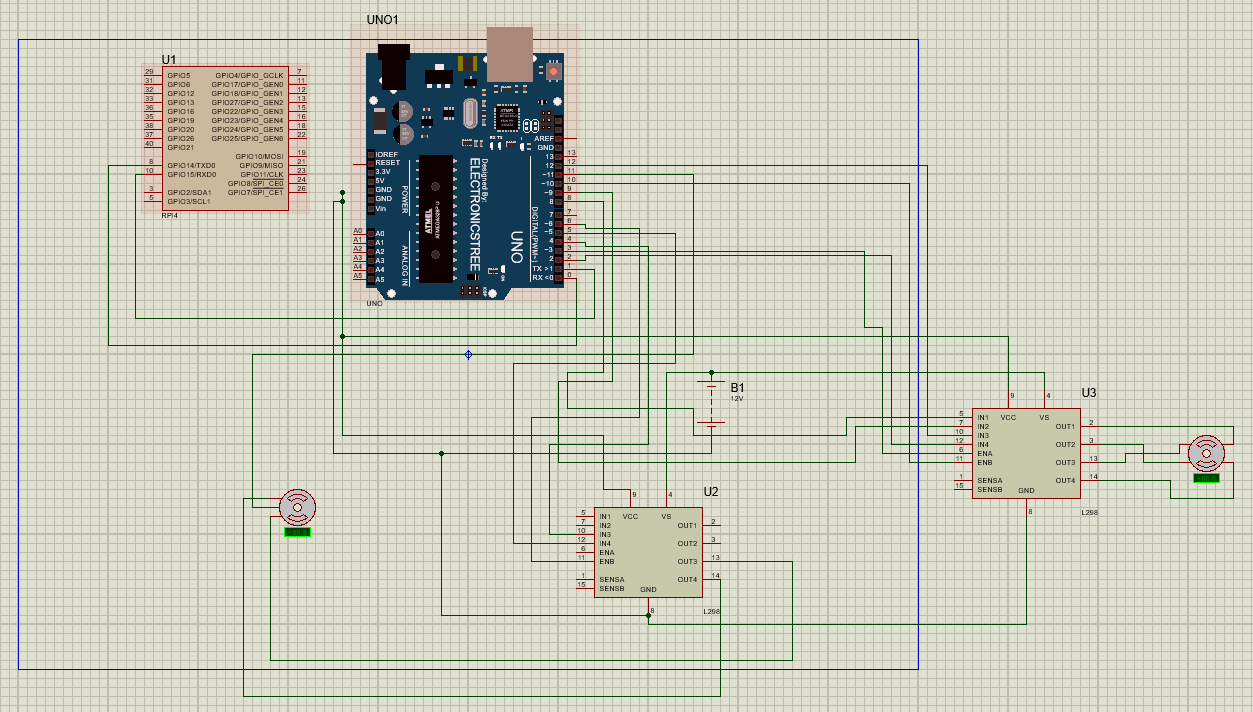
\includegraphics[width=\columnwidth]{figures/m1_proteus_circuit.png}}
  \caption{Proteus circuit simulation of the electrical architecture.
    Raspberry~Pi~4 (U1, top-left) communicates with Arduino~UNO (UNO1) via
    serial; two L298N H-bridge modules (U2, U3) drive the stepper motors;
    12~V battery (B1) provides main power; servo motor (right) handles
    column selection.}
  \label{fig:circuit}
\end{figure}

% ─────────────────────────────────────────────────────────────────────────────
\section{Mechanical Design}
\label{sec:mech}
% ─────────────────────────────────────────────────────────────────────────────

The mechanical assembly was modeled in SolidWorks. The design features a magazine
holding a stack of tokens of one color mounted over a sliding channel (Path.SLDPRT).
A DC motor drives a disk end-effector (Motor~disk.SLDPRT) that pushes the
bottom token from the magazine through the slide toward the Connect-4 board.
An SG90 micro-servo controls a gate that covers unwanted columns, ensuring the
released token is directed into the selected column only. The base
(Base.SLDPRT) and the tunnel-and-base assembly (Assem~1) provide the structural
frame securing the board and the dispensing mechanism in a fixed geometric
relationship.

This mechanism requires that the arm traverse a single horizontal axis: the
column-selection gate performs the lateral work while the pusher mechanism
provides the ejection force. This is consistent with the design guidance
from~\cite{Abarkan2024}, which demonstrates that only one active translational
axis is necessary for Connect-4 column selection.

% ─────────────────────────────────────────────────────────────────────────────
\section{Image Processing Pipeline}
\label{sec:pipeline}
% ─────────────────────────────────────────────────────────────────────────────

The processing pipeline is implemented in Python using OpenCV~4.x.
All operations listed below were executed and their outputs saved to
PNG files, which were directly inspected for this report.

\subsection{Input Image}

The pipeline input is a single overhead RGB photograph of a Connect-4 board
with red and yellow tokens in a partially played game state
(Fig.~\ref{fig:original}). The board occupies most of the frame, taken against
a white background under even artificial lighting.

\begin{figure}[htbp]
  \centerline{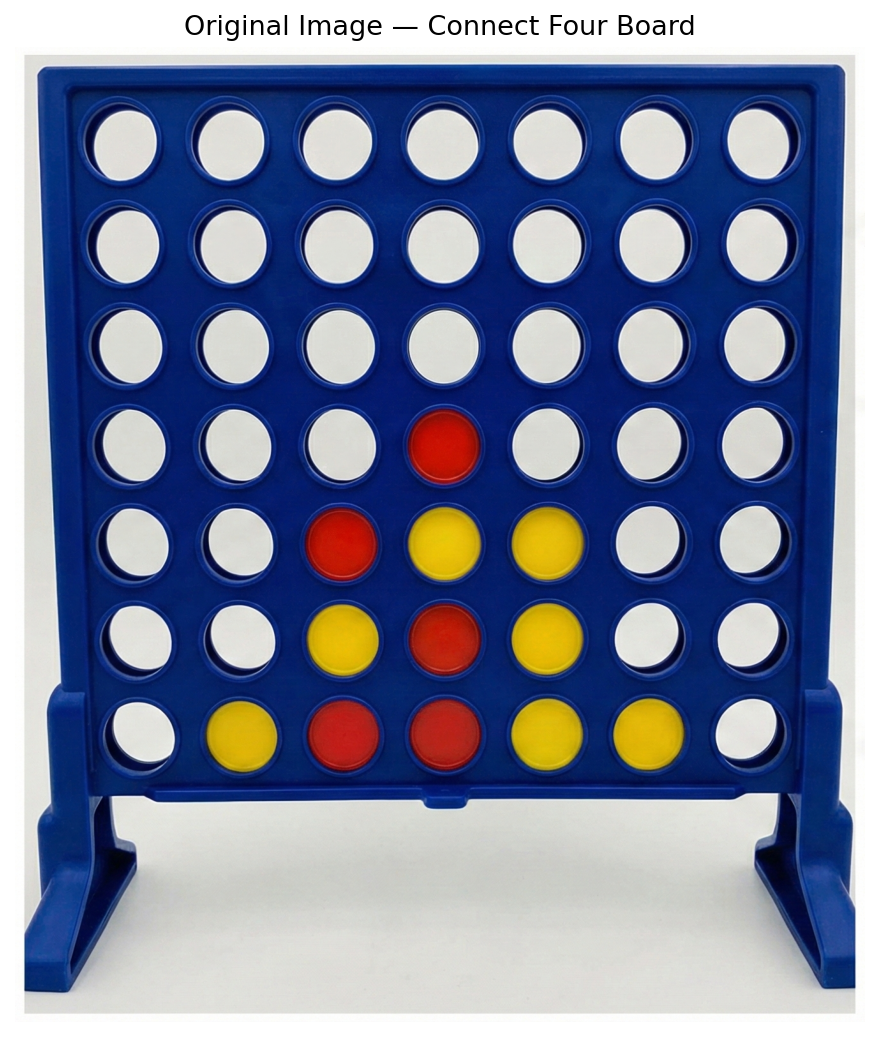
\includegraphics[width=0.70\columnwidth]{figures/m2_input_board.png}}
  \caption{Input image: Connect-4 board in a partially played state (7 columns,
    6 rows). Red and yellow tokens are present in the lower rows.}
  \label{fig:original}
\end{figure}

\subsection{Geometric Transformations}

\subsubsection{Rotation}

Camera angular offset is corrected by affine rotation. For an image domain
\(\Omega\) with center \((c_x, c_y)\), rotation by angle \(\theta\) is:
\begin{equation}
  \begin{bmatrix} x' \\ y' \end{bmatrix}
  =
  \begin{bmatrix} \cos\theta & -\sin\theta \\
                  \sin\theta &  \cos\theta \end{bmatrix}
  \begin{bmatrix} x - c_x \\ y - c_y \end{bmatrix}
  +
  \begin{bmatrix} c_x \\ c_y \end{bmatrix}.
  \label{eq:rotation}
\end{equation}
Applied at \(\theta = 15^{\circ}\), nearest-neighbor (NN) interpolation produces
jagged circular-cell boundaries, whereas bilinear interpolation averages surrounding
pixel intensities and produces smooth boundaries
(Fig.~\ref{fig:rotation}).

\begin{figure}[htbp]
  \centerline{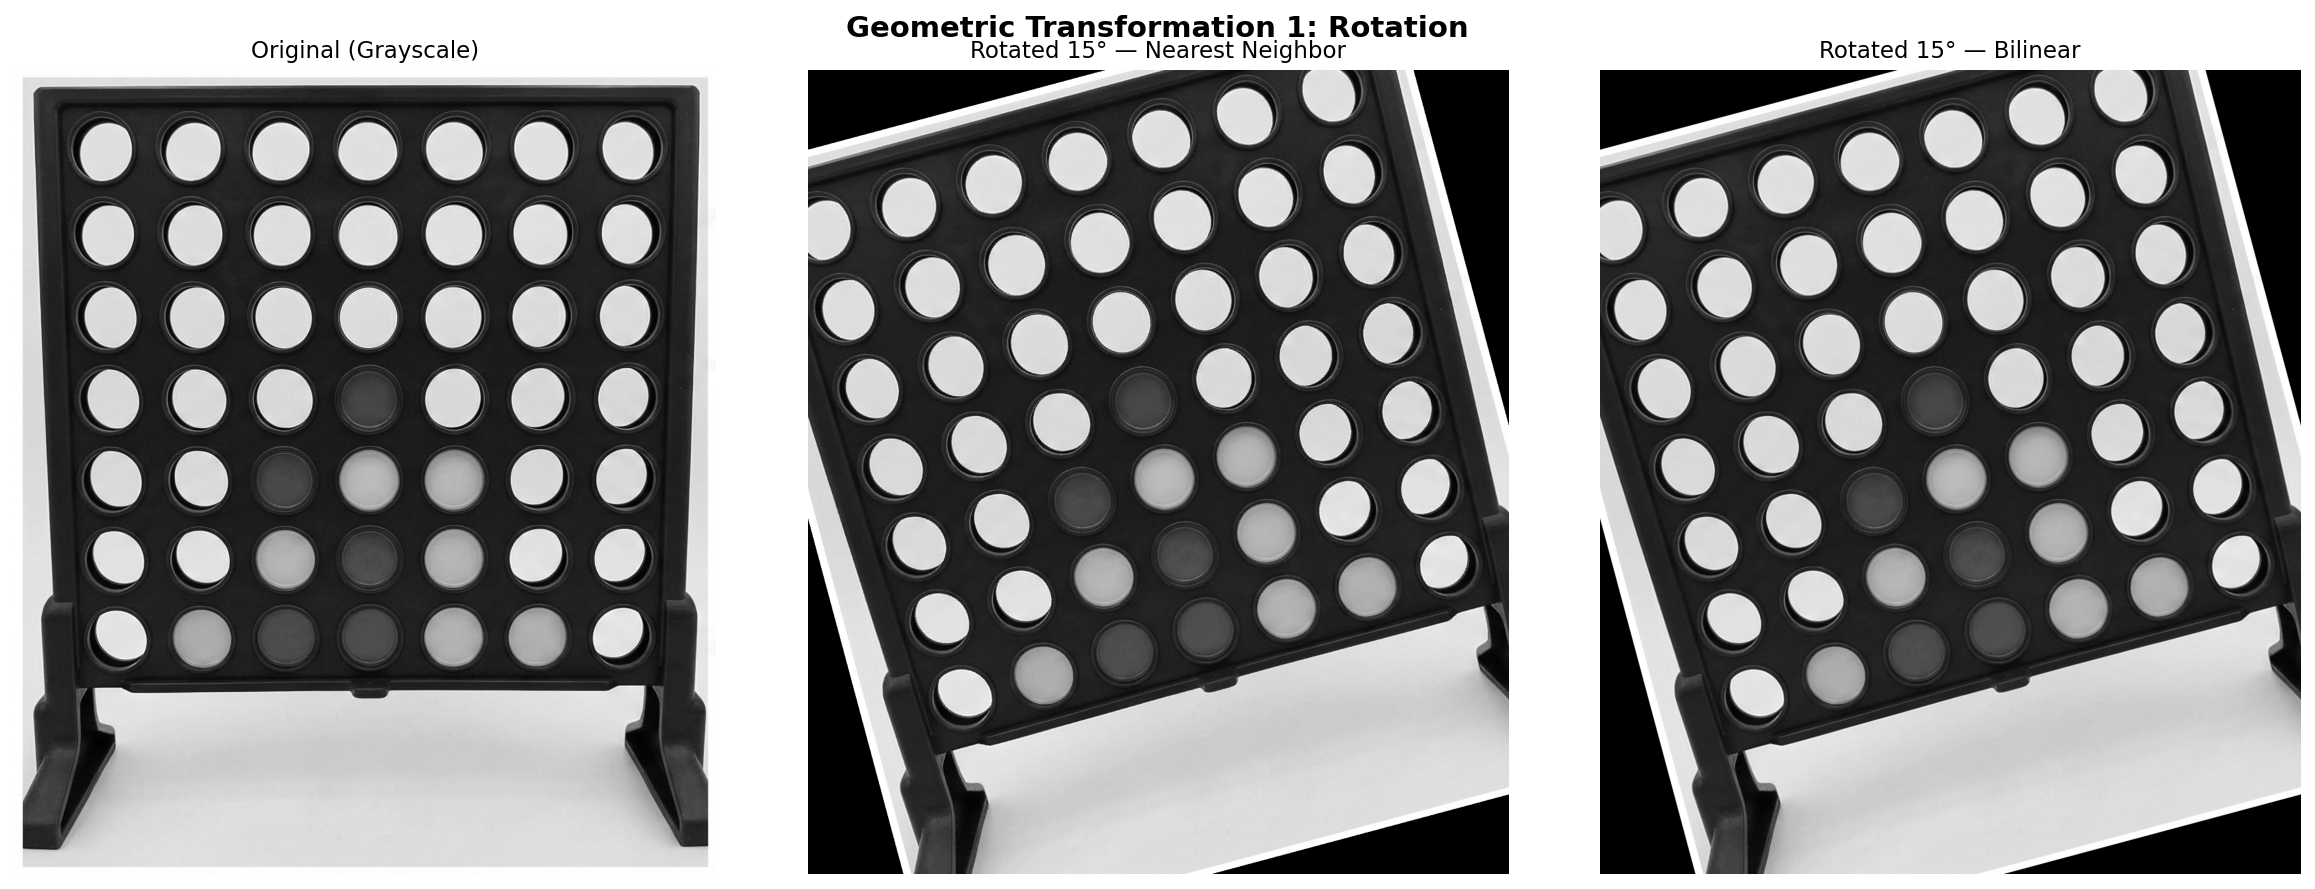
\includegraphics[width=\columnwidth]{figures/m2_rotation_comparison.png}}
  \caption{Rotation comparison at \(15^{\circ}\): (left) grayscale original;
    (center) rotated — nearest-neighbor showing aliased boundaries;
    (right) rotated — bilinear showing smooth boundaries.}
  \label{fig:rotation}
\end{figure}

\subsubsection{Perspective Warp}

Because the camera is mounted at a slight angle, orthographic flattening is
applied. A homography \(\mathbf{H} \in \mathbb{R}^{3\times3}\) maps the four
estimated board corners to an \(800 \times 800\) pixel square:
\begin{equation}
  \lambda \begin{bmatrix} u \\ v \\ 1 \end{bmatrix}
  =
  \mathbf{H}
  \begin{bmatrix} x \\ y \\ 1 \end{bmatrix}.
  \label{eq:homography}
\end{equation}
The resulting top-down orthographic view (Fig.~\ref{fig:warp}) is required for
reliable grid-index mapping of circle pixel positions. Bilinear interpolation
again yields significantly cleaner results than NN.

\begin{figure}[htbp]
  \centerline{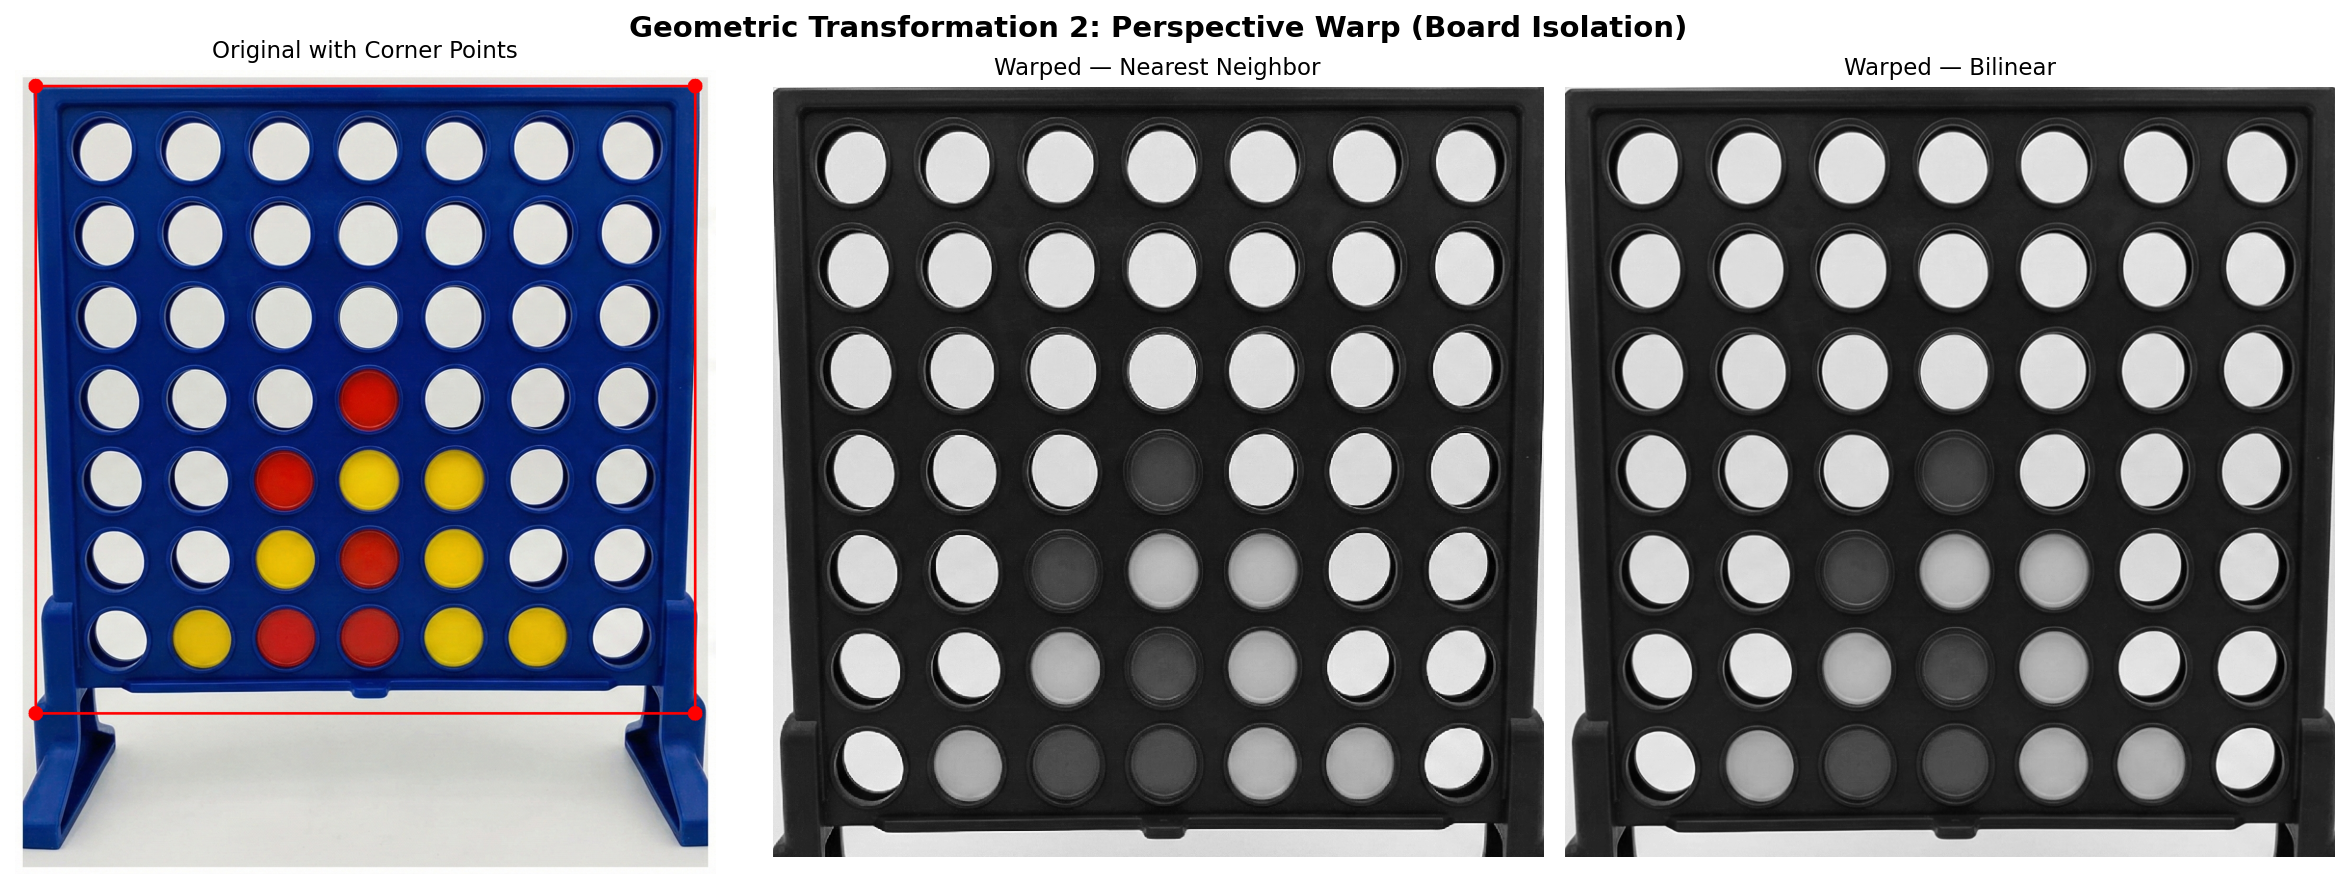
\includegraphics[width=\columnwidth]{figures/m2_perspective_warp.png}}
  \caption{Perspective warp for board isolation: (left) original with detected
    corner points; (center) warped — nearest-neighbor; (right) warped — bilinear.}
  \label{fig:warp}
\end{figure}

\subsection{Intensity Transformations}

\subsubsection{Brightness Adjustment}

The brightness transformation is the saturating shift \(I_b = \text{clip}(I + c)\),
applied with \(c = \pm 60\). Histogram analysis confirms expected behavior:
additive positive shift moves the entire pixel distribution rightward
(brightened), and subtraction moves it leftward (darkened)
(Fig.~\ref{fig:brightness}).

\begin{figure}[htbp]
  \centerline{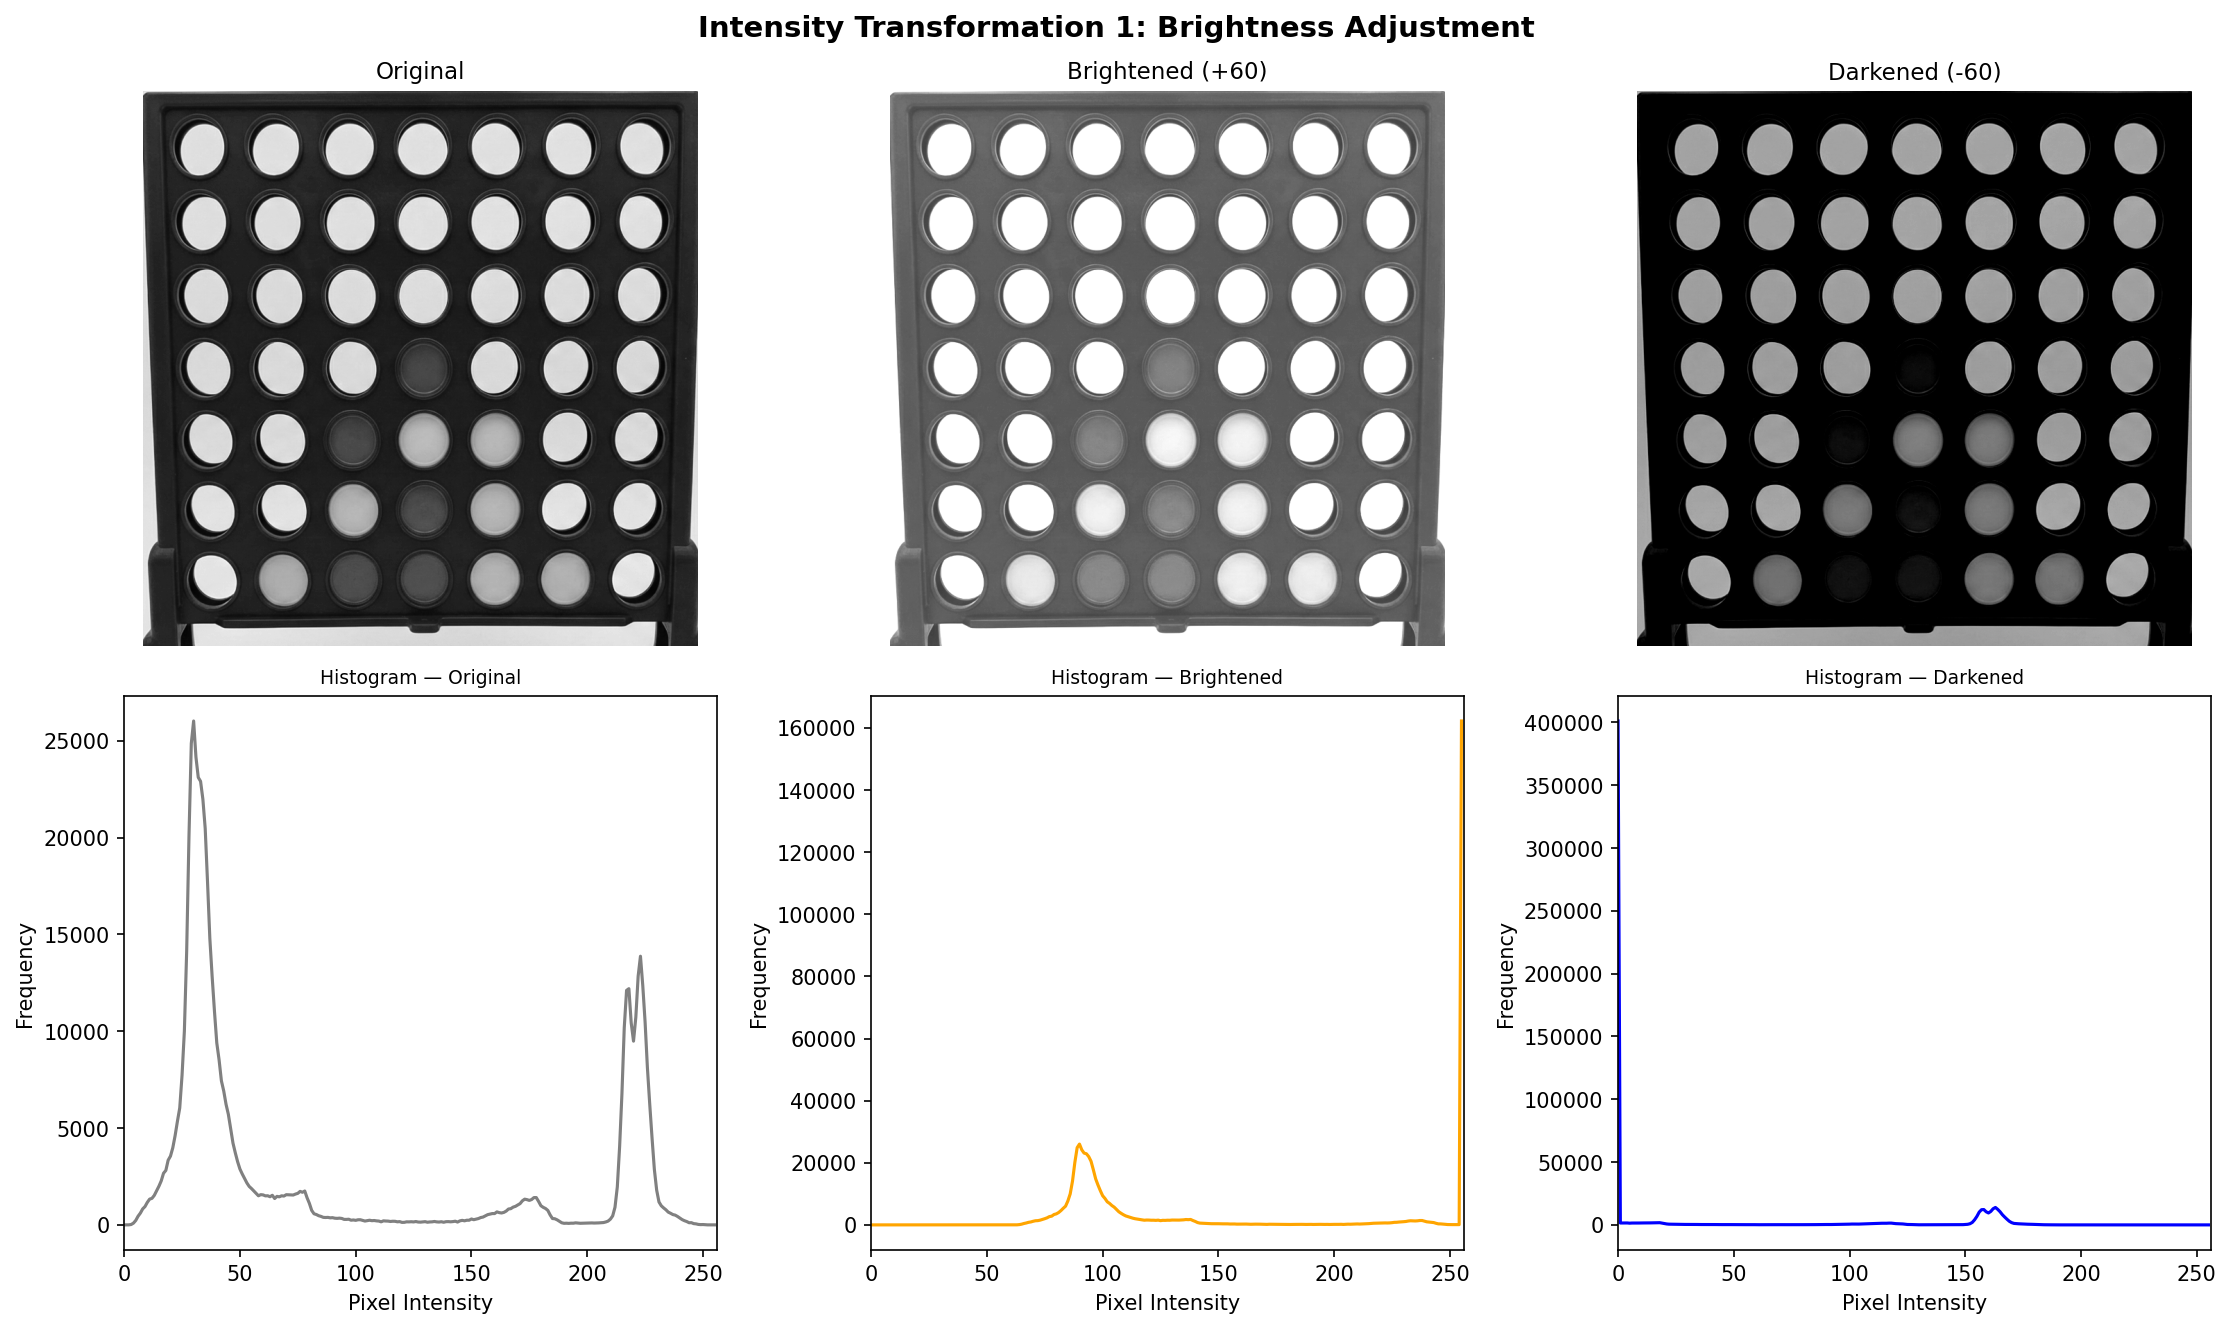
\includegraphics[width=\columnwidth]{figures/m2_brightness_adjustment.png}}
  \caption{Brightness adjustment (\(c = \pm 60\)) with corresponding pixel
    intensity histograms confirming distribution shift.}
  \label{fig:brightness}
\end{figure}

\subsubsection{Contrast Enhancement}

The linear contrast stretch is \(I_c = \text{clip}(\alpha I + \beta)\), applied
at \(\alpha = 1.8\) (high contrast) and \(\alpha = 0.5\) (low contrast) with
\(\beta = 0\). The resulting histograms show expanded and compressed
intensity distributions (Fig.~\ref{fig:contrast}), confirming that the high-contrast
setting improves separation between dark empty slots and lighter tokens.

\begin{figure}[htbp]
  \centerline{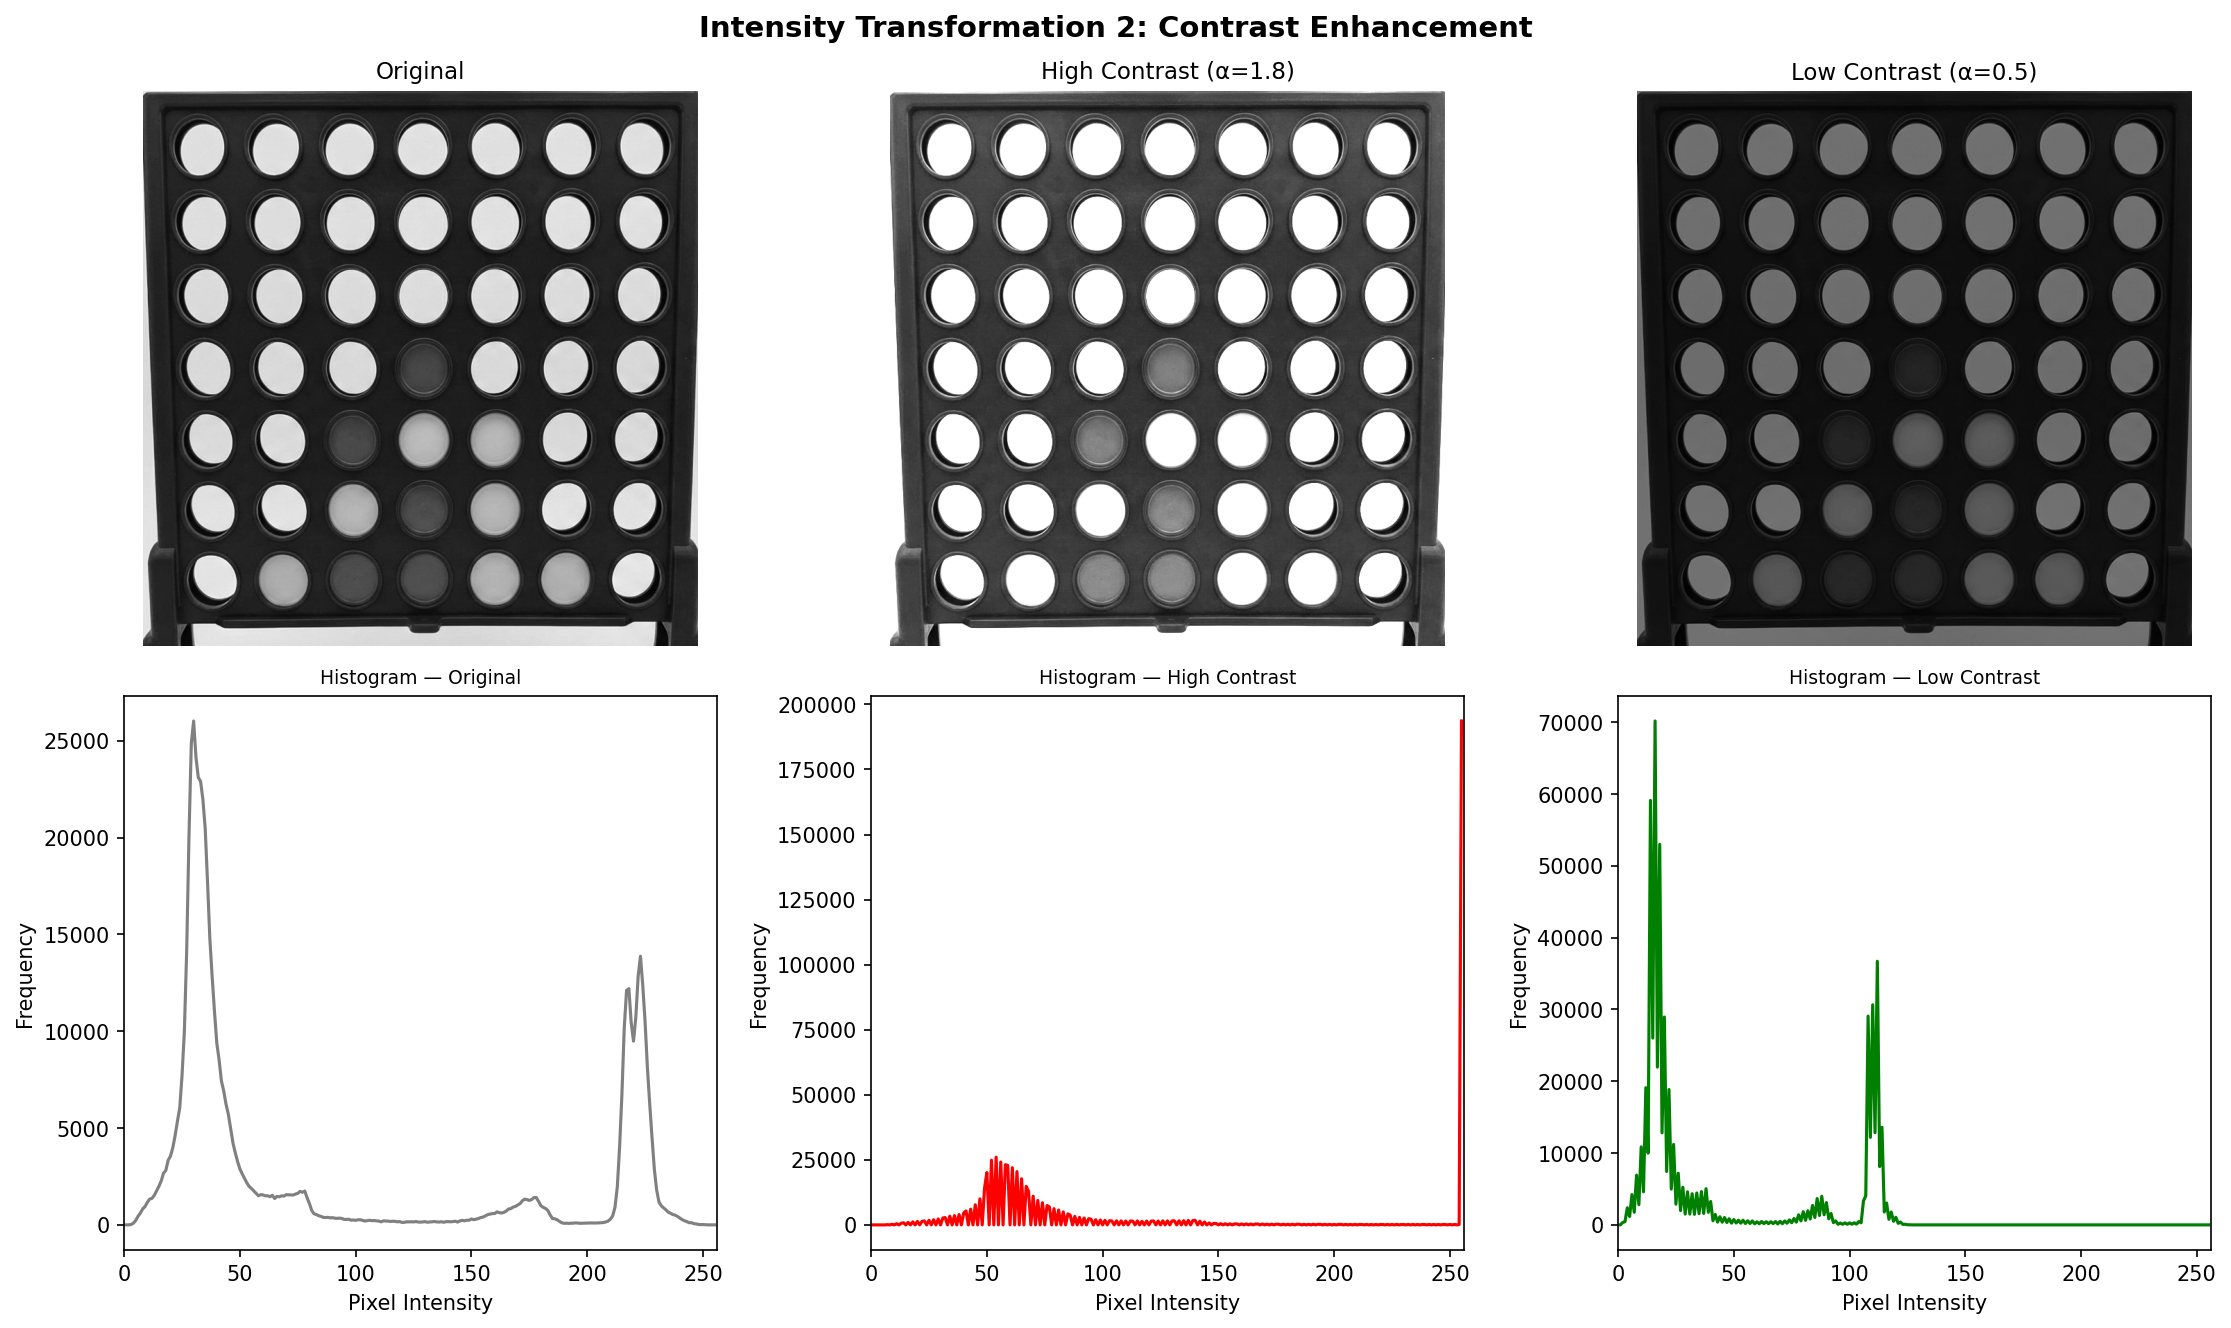
\includegraphics[width=\columnwidth]{figures/m2_contrast_scaling.png}}
  \caption{Contrast scaling at \(\alpha = 1.8\) and \(\alpha = 0.5\) with
    corresponding histograms showing distribution expansion and compression.}
  \label{fig:contrast}
\end{figure}

\subsection{Smoothing}

Camera sensor noise is suppressed by Gaussian filtering, modeled as weighted
local averaging:
\begin{equation}
  I_G(x,y) = \sum_{i=-k}^{k} \sum_{j=-k}^{k} G_\sigma(i,j)\, I(x-i,\,y-j),
  \label{eq:gaussian}
\end{equation}
where \(G_\sigma\) is normalized to unit sum. Kernels at
\(3\times3\), \(5\times5\), and \(7\times7\) were evaluated and compared to a
uniform box filter (Fig.~\ref{fig:smoothing}). As kernel size increases,
high-frequency noise is progressively suppressed but fine edge detail is
attenuated. A \(5\times5\) Gaussian kernel was selected as the operating
point, providing adequate noise suppression while preserving the circular
cell boundaries needed for downstream segmentation.

\begin{figure}[htbp]
  \centerline{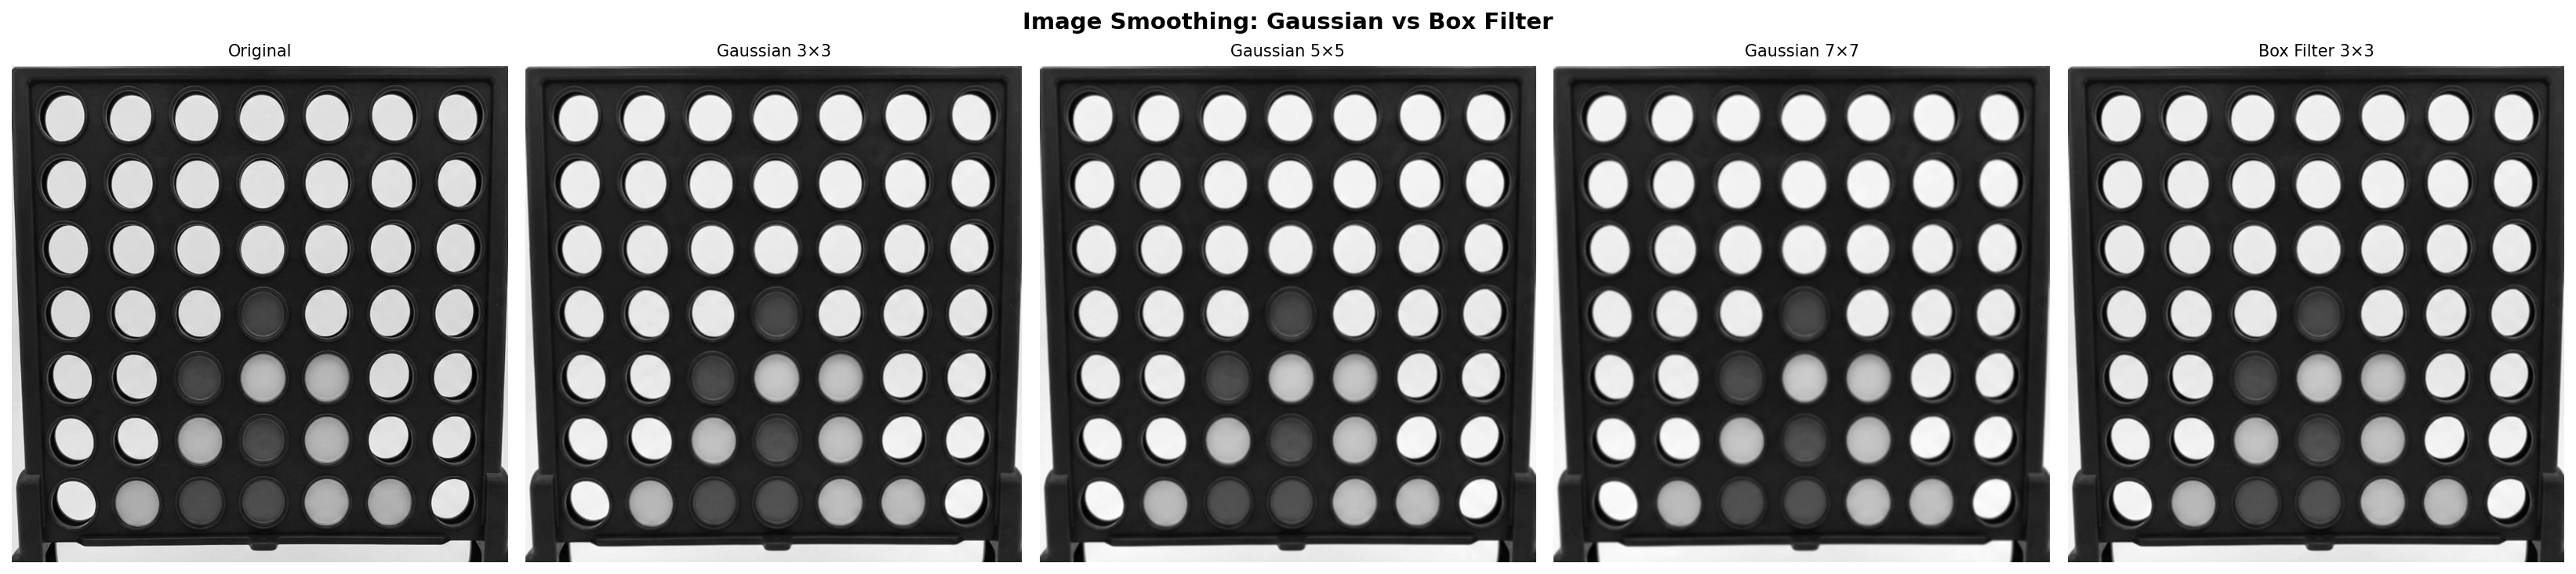
\includegraphics[width=\columnwidth]{figures/m2_smoothing_comparison.png}}
  \caption{Smoothing comparison: original (warped, grayscale),
    Gaussian \(3\times3\), \(5\times5\), \(7\times7\), and box filter \(3\times3\).
    The \(5\times5\) Gaussian offers the best trade-off between noise attenuation
    and boundary preservation.}
  \label{fig:smoothing}
\end{figure}

% ─────────────────────────────────────────────────────────────────────────────
\section{Feature Extraction and Closed-Loop Control}
\label{sec:features}
% ─────────────────────────────────────────────────────────────────────────────

Two scalar image features are extracted per processed frame and transmitted
to the Arduino via a two-byte serial protocol at 9600 baud.

\subsection{Feature 1: Mean Board Brightness}

The mean pixel intensity of the perspective-warped board region is computed as:
\begin{equation}
  \mu_b = \frac{1}{|\Omega_w|} \sum_{(x,y)\in\Omega_w} I_w(x,y),
  \label{eq:mean_brightness}
\end{equation}
where \(\Omega_w\) is the \(800\times800\) warped board domain and \(I_w\)
is the grayscale warped image. The measured value for the test image is
\(\mu_b = 91.19\). This maps to a motor speed setpoint as:
\begin{equation}
  \text{Speed\%} = \frac{\mu_b}{255} \times 100 \approx 35\%\ \text{PWM duty cycle},
  \label{eq:speed_map}
\end{equation}
where brighter board conditions correspond to higher confidence and faster
movement, while low-light conditions attenuate the duty cycle.

\subsection{Feature 2: Board Rotation Angle}

The angular offset of the board with respect to the image frame is extracted
from the affine rotation matrix:
\begin{equation}
  \phi = \arctan2\!\bigl(M_{10},\,M_{00}\bigr),
  \label{eq:angle}
\end{equation}
where \(M_{00} = \cos\theta\) and \(M_{10} = \sin\theta\) are elements of
the rotation matrix. The warp correction angle of \(15^{\circ}\) is
extracted and mapped to motor direction: positive values correspond to
clockwise correction, negative values to counter-clockwise correction.

\subsection{Serial Protocol}

The two feature values are serialized as raw bytes. The Pi transmits them
over USB serial; the Arduino reads two consecutive bytes in each loop cycle
using \texttt{Serial.read()} and writes the first byte as servo angle~1 and
the second as servo angle~2.

% ─────────────────────────────────────────────────────────────────────────────
\section{Embedded Platform Benchmarking}
\label{sec:bench}
% ─────────────────────────────────────────────────────────────────────────────

Each pipeline operation was benchmarked over 100 iterations on both the
Raspberry~Pi~4 and a laptop. Table~\ref{tab:bench} reports the mean time
per operation. Output image quality is bit-for-bit identical on both platforms;
the limitation of the Raspberry~Pi is temporal throughput, not spatial accuracy.

\begin{table}[htbp]
  \caption{Per-Operation Execution Time: Raspberry Pi 4 vs.\ Laptop (100-iteration mean)}
  \label{tab:bench}
  \begin{center}
    \begin{tabular}{lrr}
      \toprule
      \textbf{Operation} & \textbf{Pi 4 (ms)} & \textbf{Laptop (ms)} \\
      \midrule
      Rotation (bilinear)     & 8.468 & 3.273 \\
      Perspective warp        & 3.596 & 1.768 \\
      Brightness +60          & 0.734 & 0.888\textsuperscript{a} \\
      Contrast \(\alpha=1.8\) & 1.111 & 0.201 \\
      Gaussian blur 5\(\times\)5 & 0.757 & 0.097 \\
      \bottomrule
      \multicolumn{3}{l}{\textsuperscript{a}Pi faster than laptop for this saturating-add
        operation, likely due to ARM NEON SIMD efficiency.}
    \end{tabular}
  \end{center}
\end{table}

% ─────────────────────────────────────────────────────────────────────────────
\section{System Component Cost}
\label{sec:cost}
% ─────────────────────────────────────────────────────────────────────────────

Table~\ref{tab:bom} lists the verified hardware components and their costs
in Egyptian Pounds (EGP) at procurement time.

\begin{table}[htbp]
  \caption{Hardware Bill of Materials}
  \label{tab:bom}
  \begin{center}
    \begin{tabular}{lrr}
      \toprule
      \textbf{Component} & \textbf{Qty} & \textbf{Total (EGP)} \\
      \midrule
      Raspberry Pi 4 (4\,GB)  & 1 & 5,950 \\
      Arduino Uno              & 1 &   450 \\
      Pi Camera V2             & 1 & 2,150 \\
      NEMA 17 stepper motor    & 2 &   880 \\
      L298N H-bridge driver    & 2 &   170 \\
      SG90 micro-servo         & 1 &    85 \\
      12\,V 5\,A power supply  & 1 &   300 \\
      Wires \& breadboard      & 1 &   150 \\
      \midrule
      \textbf{Total}           &   & \textbf{10,135} \\
      \bottomrule
    \end{tabular}
  \end{center}
\end{table}

% ─────────────────────────────────────────────────────────────────────────────
\section{Limitations and Future Work}
\label{sec:future}
% ─────────────────────────────────────────────────────────────────────────────

The current implementation covers image acquisition, preprocessing, and
feature-based motor command generation. The following subsystems
are identified as remaining work:

\begin{enumerate}
\item \emph{HSV color segmentation}: Cell-level token-color classification
  using the HSV pipeline described in~\cite{Zubek2021} and~\cite{Park2024}
  has not yet been implemented.
\item \emph{Game AI}: The minimax algorithm with alpha-beta pruning for
  optimal move selection is not yet implemented.
\item \emph{Full motor firmware}: The NEMA~17 stepper control firmware
  (step direction, speed, distance) was not recovered in the workspace
  beyond the servo validation sketch.
\item \emph{Pipeline validation breadth}: The current pipeline has been
  validated on a single board image. Multi-scene, multi-lighting validation
  is required before deployment.
\item \emph{Real-time integration}: End-to-end latency
  \(T_\text{loop} = t_c + t_p + t_s\) (capture + processing + serial) must
  be profiled under operating conditions on the Raspberry~Pi.
\end{enumerate}

% ─────────────────────────────────────────────────────────────────────────────
\section{Conclusion}
\label{sec:conclusion}
% ─────────────────────────────────────────────────────────────────────────────

This paper presented the image processing pipeline and hardware architecture
of a Vision-Based Connect-4 Robot through Milestone~2. The Python/OpenCV
pipeline—comprising orthographic warp, brightness normalization, and
Gaussian smoothing—executes reliably on a Raspberry~Pi~4, producing
bit-for-bit identical outputs to a laptop at latencies ranging from
0.73~ms to 8.47~ms per operation. Two scalar features extracted from
each processed frame provide a practical interface to the Arduino-based
actuation stage. The SolidWorks mechanical model and Proteus circuit
simulation establish a verified hardware foundation for subsequent
integration with token-color segmentation and game-solving logic.

\section*{Acknowledgment}

The authors acknowledge the Department of Mechatronics Engineering,
German University in Cairo, for laboratory access and supervision.

\bibliographystyle{IEEEtran}
\bibliography{references}

\end{document}
